%%%%%%%%%%%%%%%%%%%%%%%%%%%%%%%%%%%%%%%%%%%%%%%%%%%%%%%%%%%%
\documentclass[9pt,            % Schriftgröße {{{
               a4paper,         % A4
               landscape,
               halfparskip,
               oneside,         % Einseitig
               DIV94,           % Papiergröße
              ]{scrartcl} %%% }}}
%%%%%%%%%%%%%%%%%%%%%%%%%%%%%%%%%%%%%%%%%%%%%%%%%%%%%%%%%%%%

%%%%%%%%%%%%%%%%%%%%%%%%%%%%%%%%%%%%%%%%%%%%%%%%%%%%%%%%%%%%
%%% Pakete {{{
\usepackage[utf8]{inputenc}         % Umlaute etc.
\usepackage[T1]{fontenc}            % T1-kodierte Fonts
\usepackage{ae,aecompl}             % Kodierung für PDF
\usepackage{ngerman}                % Deutsche Trennungen,
                                    % dt. Begriffe
\usepackage{setspace}               % Single- oder Onehalfspacing
\setcounter{tocdepth}{4}            % 4 Hirarchien im Inhaltsv.
\usepackage{times}                  % Times als Schrift
\usepackage{amsmath,amssymb,amstext}% Mathematische Symbole
\usepackage{exscale}                % Skalierung von Summen-c und Int.-zeichen
\usepackage{url}                    % Darstellung von URLs
\usepackage{calc}

%%% Optional, je nach Dokument
% \usepackage{listings}             % Quelltext-Listings
% \usepackage{units}                % Technische Units
% \usepackage{psfrag}               % Ersetzts PS-Schriften
  \usepackage{color}                % Farben in LaTeX
% \usepackage{floatflt}             % Textumflossene Bilder...
% \usepackage{picins}               % Textumflossene Bilder
  \usepackage{textcomp}             % Spezielle Zeichen
  \usepackage{gensymb}              % Spezielle Zeichen
% \usepackage{eurosym}              % Euro-Symbol
% \usepackage{currvita}             % Befehle für CVs
  \usepackage{ifpdf}                % Wird ein PDF erstellt?

%%% Layout
\usepackage{scrpage2}               % KOMA-Überschriften und -Fußzeilen.
%%% }}}
%%%%%%%%%%%%%%%%%%%%%%%%%%%%%%%%%%%%%%%%%%%%%%%%%%%%%%%%%%%%

%%%%%%%%%%%%%%%%%%%%%%%%%%%%%%%%%%%%%%%%%%%%%%%%%%%%%%%%%%%%
%%% PDF {{{

\ifpdf
  \usepackage[pdftex]{graphicx}
  \DeclareGraphicsExtensions{.pdf}
  \pdfcompresslevel=9
  \usepackage[%
    pdftex=true,
    backref=true,
    colorlinks=true,
    bookmarks=true,
    breaklinks=true,
    linktocpage=true,
    bookmarksopen=false,
    bookmarksnumbered=false,
    pdfpagemode=None
  ]{hyperref}
  \hypersetup{
    pdftitle={},
    pdfauthor={Julius Plenz},
    pdfsubject={},
    pdfcreator={LaTeX2e and pdfLaTeX},
    pdfproducer={},
    pdfkeywords={}
  }
\else
  \usepackage[dvips]{graphicx}
  \DeclareGraphicsExtensions{.eps}
  % \usepackage[%
  %   dvips,
  %   breaklinks=true,
  %   colorlinks=false
  % ]{hyperref}
\fi

%%% }}}
%%%%%%%%%%%%%%%%%%%%%%%%%%%%%%%%%%%%%%%%%%%%%%%%%%%%%%%%%%%%

%%%%%%%%%%%%%%%%%%%%%%%%%%%%%%%%%%%%%%%%%%%%%%%%%%%%%%%%%%%%
%%% Eigene Funktionen {{{
%%% Beispiel:  \bild{200pt}{foo}{That's a foo\ldots}
\newcommand{\bild}[3]{
  \begin{figure}
    \includegraphics[width=#1, keepaspectratio=true]{#2}
    \caption{#3}
    \label{#2}
  \end{figure}
}

%% \floatimg{filename}{caption+label}{r/l}{8cm}
\newcommand{\floatimg}[4]{
  \piccaption{#2}
  \parpic[#3]{\includegraphics[width=#4]{#1}}
}

\newcommand{\platz}{\vspace{-4.5ex}}
\def \breiteErsteSpalte {7cm}
\def \breiteZweiteSpalte {9cm}
\def \breiteDritteSpalte {11cm}

\usepackage{mathtools}
\newcommand{\textover}[2]{\stackrel{\mathclap{\normalfont\mbox{#1}}}{#2}}


%%% }}}
%%%%%%%%%%%%%%%%%%%%%%%%%%%%%%%%%%%%%%%%%%%%%%%%%%%%%%%%%%%%

%%%%%%%%%%%%%%%%%%%%%%%%%%%%%%%%%%%%%%%%%%%%%%%%%%%%%%%%%%%%
%%% Pagestyle {{{
% \pagestyle{scrheadings}
% \pagestyle{fancyhdrs}
  \pagestyle{empty}
%%% }}}
%%%%%%%%%%%%%%%%%%%%%%%%%%%%%%%%%%%%%%%%%%%%%%%%%%%%%%%%%%%%

%%%%%%%%%%%%%%%%%%%%%%%%%%%%%%%%%%%%%%%%%%%%%%%%%%%%%%%%%%%%
%%% Seitenkopf- und -Fußzeilen {{{
 \automark[subsection]{section} % \left- und \rightmark bekommen Inhalt
%%% Oben: Links, Mitte, Rechts
 \ihead[]{}
 \chead[]{}
 \ohead[]{}
%%% Unten: Links, Mitte, Rechts
 \ifoot[]{}
 \cfoot[]{}
 \ofoot[]{}
%%% }}}
%%%%%%%%%%%%%%%%%%%%%%%%%%%%%%%%%%%%%%%%%%%%%%%%%%%%%%%%%%%%

\usepackage{tikz}
\usetikzlibrary{shapes,decorations,shadows}

%%%%%%%%%%%%%%%%%%%%%%%%%%%%%%%%%%%%%%%%%%%%%%%%%%%%%%%%%%%%
%%% Sonstiges {{{
% \setlength{\parindent}{17pt}      % Einzug 17pt,
% \setlength{\parskip}{2pt}         % keine Leerzeilen.

% \textwidth      127mm             % Textbreite
% \textheight     235mm             % Texthöhe
% \topmargin     -5mm               % Abstand oben
% \oddsidemargin  7mm               % Abstand Links, onepage

%\onehalfspacing                    % Zeilenabstand: Bei korrektur,
 \singlespacing                     % bei Abgabe

% Punkt- und Komma Abstände bei Tausendern/
% Dezimalzahlen ans deutsche anpassen!
 \mathcode`,="013B
 \mathcode`.="613A

 \setlength{\emergencystretch}{2em} % Notfallsstreckung
 \addtolength{\voffset}{10pt}

% Kommandoänderungen
 \renewcommand{\figurename}{Abb.} % Bildunterschriften: Abb. anstatt Fig.
%\renewcommand*{\cvheadingfont}{\raggedleft\Huge\bfseries} % CV: Überschriften
%%% }}}
%%%%%%%%%%%%%%%%%%%%%%%%%%%%%%%%%%%%%%%%%%%%%%%%%%%%%%%%%%%%


% Platz links, über und unter Überschriften ändern
%\usepackage{titlesec}
%\titlespacing*{\subsection}{0pt}{5.5ex plus 1ex minus .2ex}{4.3ex plus .2ex}


\begin{document}

%%%%%%%%%%%%%%%%%%%%%%%%%%%%%%%%%%%%%%%%%%%%%%%%%%%%%%%%%%%%
%%% Inhalt {{{


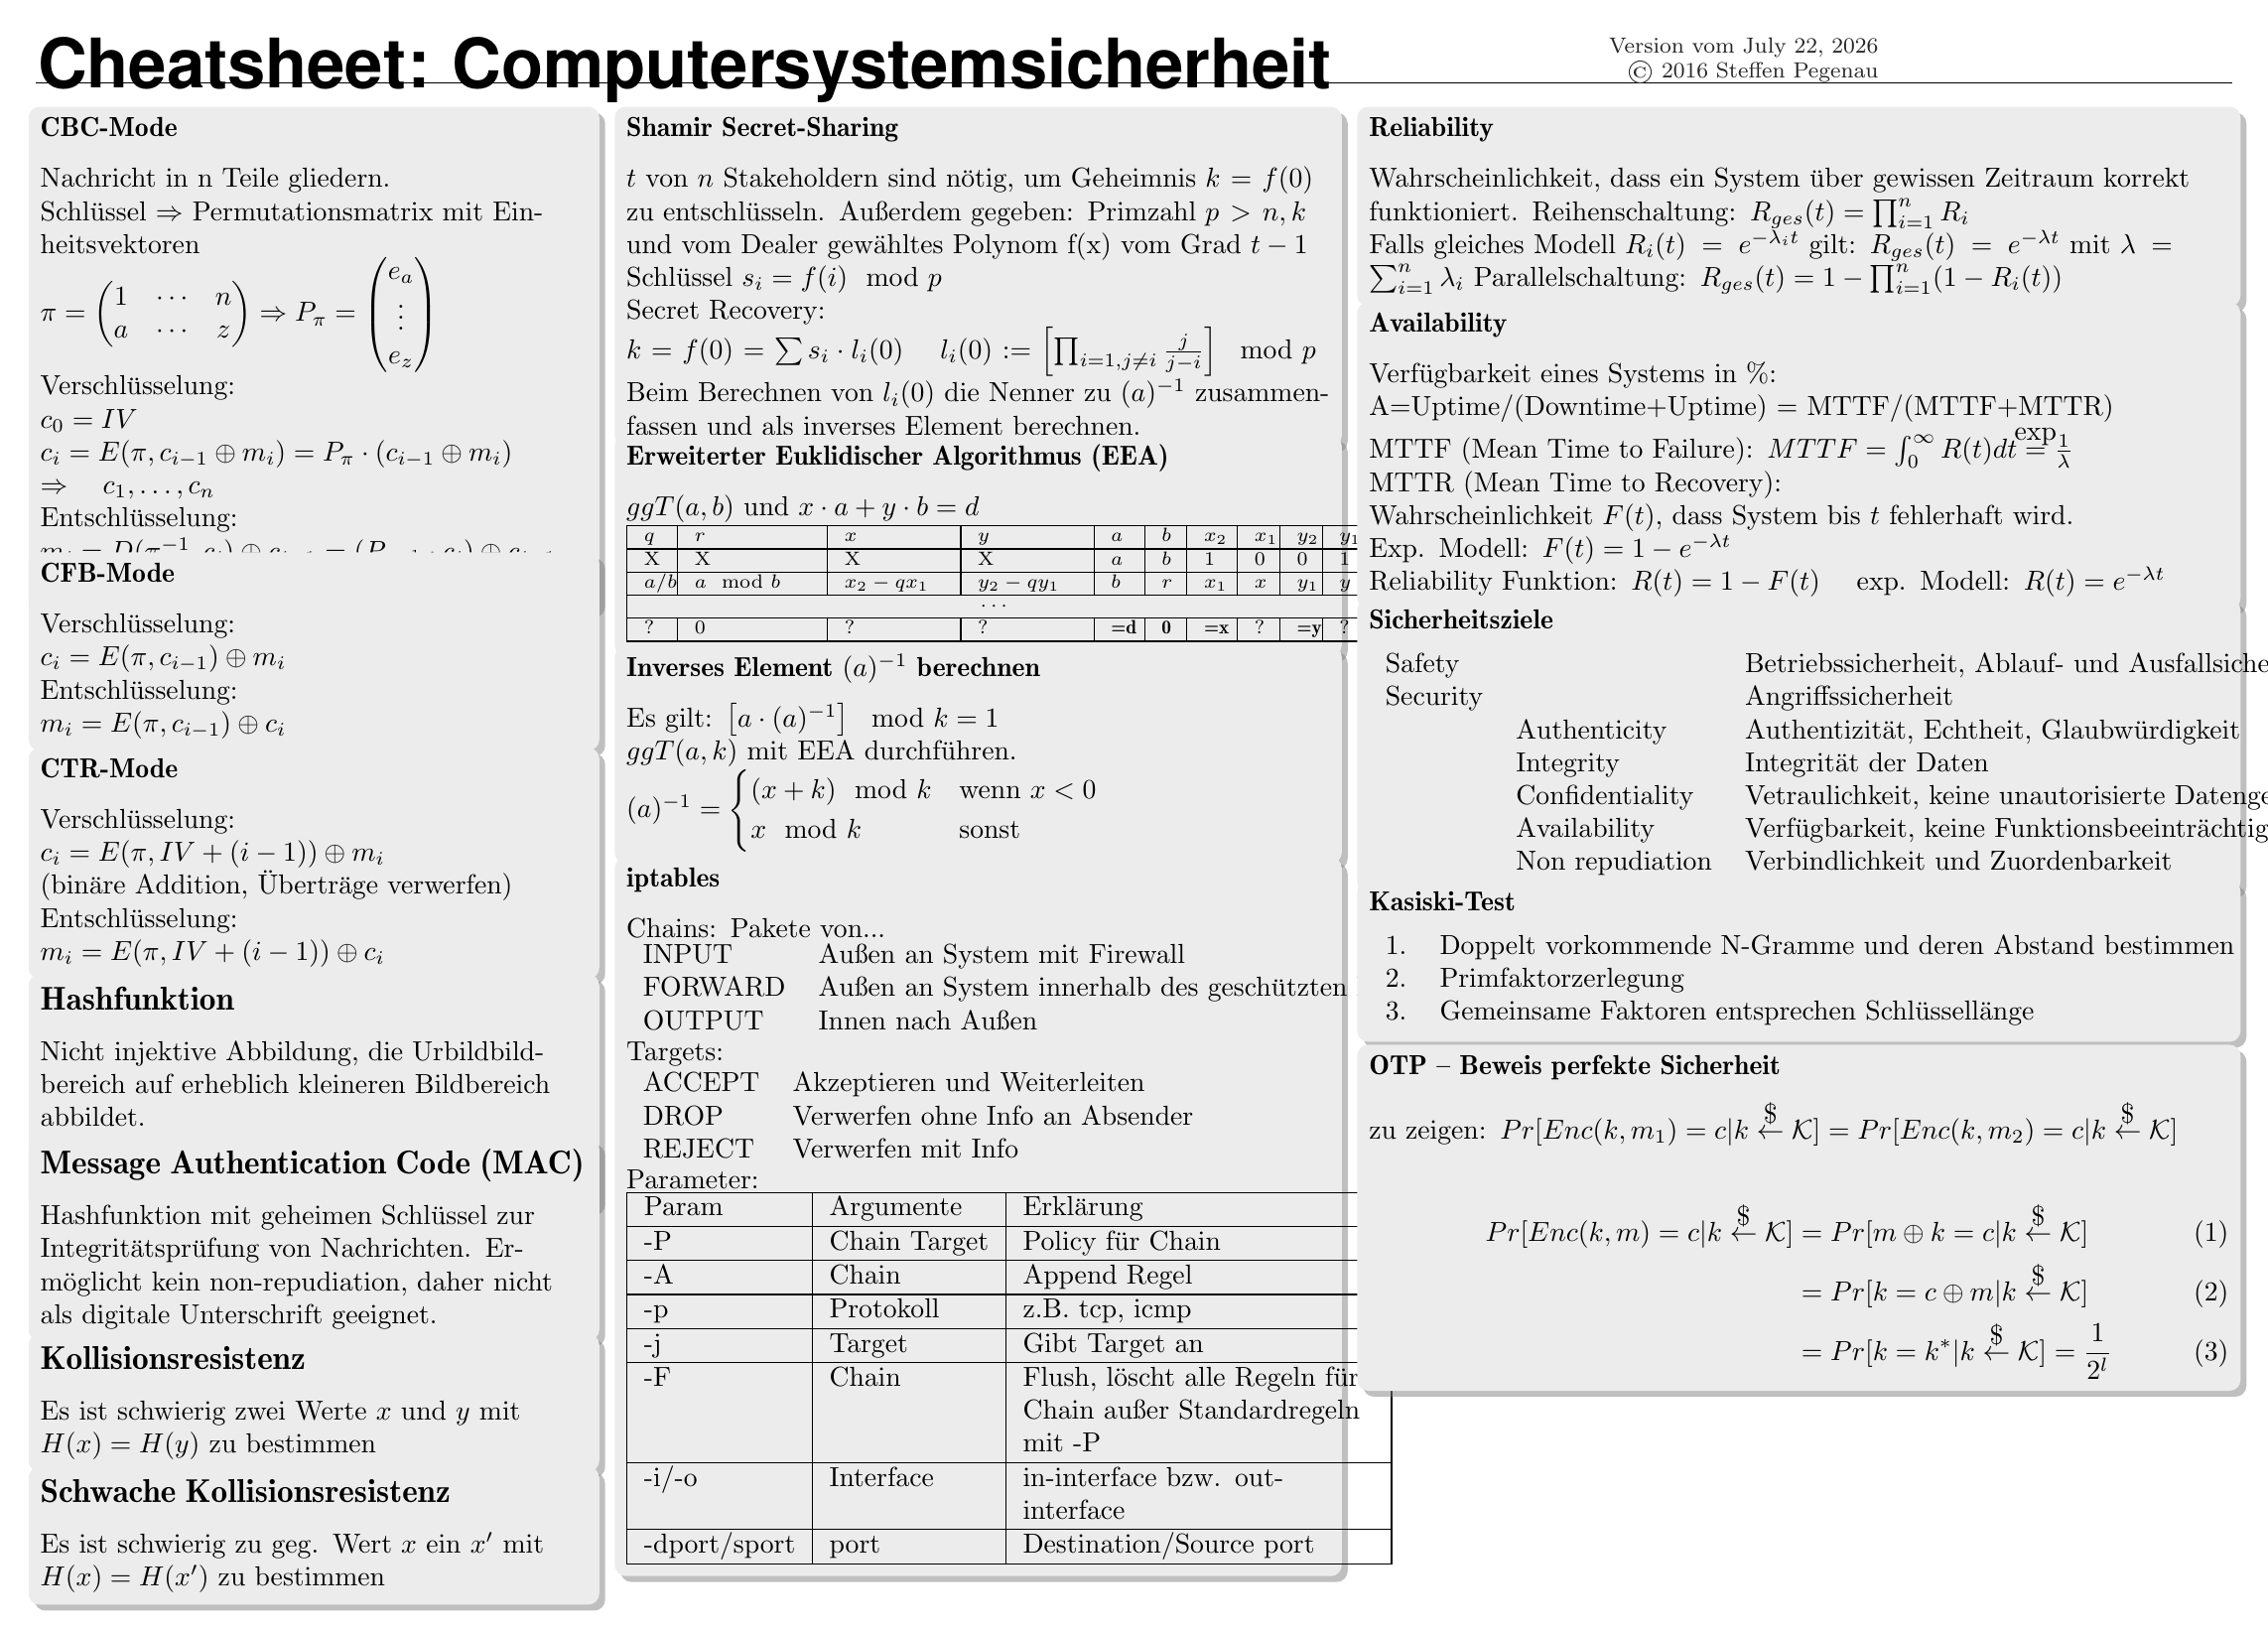
\begin{tikzpicture}
  \draw (0,1) node[anchor=north west,font=\Huge\bf\fontfamily{phv}\selectfont]{Cheatsheet: Computersystemsicherheit}
  (.1cm,.3cm) -- (28.2cm,.3cm)
  ([xshift=1mm]23.7cm,.7cm)
  node[font=\footnotesize,color=black!85,anchor=north east]{
    \copyright{} 2016 Steffen Pegenau
  }
  ++(0,.3cm)
  node[font=\footnotesize,color=black!85,anchor=north east]{
    Version vom \today
  }
  ;
  \draw
  (0,0) node[anchor=north west,text width=\breiteErsteSpalte,rounded corners,fill=gray!15,inner sep=1ex,drop shadow]
  (linksoben)
  {
   \platz
   \subsubsection*{CBC-Mode}
    Nachricht in n Teile gliedern. \\
    Schlüssel $\Rightarrow$ Permutationsmatrix mit Einheitsvektoren\\
    $\pi = \left(
    \begin{matrix}
     1 & \cdots & n \\
     a & \cdots & z \\
    \end{matrix} \right)
    \Rightarrow
    P_\pi = \left(
    \begin{matrix}
    e_a \\
    \vdots \\
    e_z \\
    \end{matrix}
    \right) $ \\
    Verschlüsselung: \\
    $c_0 = IV$ \\
    $c_i = E(\pi, c_{i-1} \oplus m_i) = P_\pi \cdot (c_{i-1} \oplus m_i)$\\
    $\Rightarrow \quad c_1, \dots, c_n$ \\
    Entschlüsselung: \\
    $m_i = D(\pi^{-1},c_i)\oplus c_{i-1} = (P_{\pi^{-1}} \cdot c_i) \oplus c_{i-1}$\\
    mit $\pi^{-1} = \pi'$ (transponiert)
  }
  ++(0,-5.7cm) node[below right,text width=\breiteErsteSpalte,rounded corners,fill=gray!15,inner sep=1ex,drop shadow]
  {
    \platz
    \subsubsection*{CFB-Mode}
    Verschlüsselung: \\
    $c_i = E(\pi, c_{i-1} )\oplus m_i$\\
    Entschlüsselung: \\
    $m_i = E(\pi, c_{i-1}) \oplus c_i$
  }
  ++(0,-2.5cm) node[below right,text width=\breiteErsteSpalte,rounded corners,fill=gray!15,inner sep=1ex,drop shadow]
  {
    \platz
    \subsubsection*{CTR-Mode}
    Verschlüsselung: \\
    $ c_i = E(\pi, IV + (i-1)) \oplus m_i $ \\
    (binäre Addition, Überträge verwerfen) \\
    Entschlüsselung: \\
    $ m_i = E(\pi, IV + (i-1)) \oplus c_i $
  }
  ++(0, -2.9cm) node[below right,text width=\breiteErsteSpalte,rounded corners,fill=gray!15,inner sep=1ex,drop shadow]
  {
    \platz
    \subsection*{Hashfunktion}
    Nicht injektive Abbildung, die Urbildbildbereich auf erheblich kleineren Bildbereich abbildet.\\
    Speicherung von Passwörtern, Dateivalidierung
    
  }
  ++(0, -2.1cm) node[below right,text width=\breiteErsteSpalte,rounded corners,fill=gray!15,inner sep=1ex,drop shadow]
  {
    \platz
    \subsection*{Message Authentication Code (MAC)}
    Hashfunktion mit geheimen Schlüssel zur Integritätsprüfung von Nachrichten. Ermöglicht 
    kein non-repudiation, daher nicht als digitale Unterschrift geeignet.
  }
  ++(0, -2.5cm) node[below right,text width=\breiteErsteSpalte,rounded corners,fill=gray!15,inner sep=1ex,drop shadow]
  {
    \platz
    \subsection*{Kollisionsresistenz}
    Es ist schwierig zwei Werte $x$ und $y$ mit $H(x) = H(y)$ zu bestimmen
  }
  ++(0, -1.7cm) node[below right,text width=\breiteErsteSpalte,rounded corners,fill=gray!15,inner sep=1ex,drop shadow]
  {
    \platz
    \subsection*{Schwache Kollisionsresistenz}
    Es ist schwierig zu geg. Wert $x$ ein $x'$ mit $H(x) = H(x')$ zu bestimmen
  }
% Als Visualisierung brauchbar?
;
  \draw (linksoben.north west)
  ++(7.5cm,0) node[anchor=north west,text width=\breiteZweiteSpalte,rounded corners,fill=gray!15,inner sep=1ex,drop shadow]
  (zweite-spalte)
  {
    \platz
    \subsubsection*{Shamir Secret-Sharing}
    $t$ von $n$ Stakeholdern sind nötig, um Geheimnis $k = f(0)$ zu entschlüsseln. Außerdem gegeben:
    Primzahl $p>n,k$ und vom Dealer gewähltes Polynom f(x) vom Grad $t-1$ \\
    Schlüssel $s_i = f(i) \mod p$ \\
    Secret Recovery: \\
    $k = f(0) = \sum s_i \cdot l_i(0)$ \quad
    $l_i(0) := \left[\prod_{i=1,j\neq i} \frac{j}{j - i}\right] \mod p$
    Beim Berechnen von $l_i(0)$ die Nenner zu $(a)^{-1}$ zusammenfassen und als inverses
    Element berechnen.
  }
  ++(0,-4.2cm) node[below right,text width=\breiteZweiteSpalte,rounded corners,fill=gray!15,inner sep=1ex,drop shadow]
  {
    \platz
    \subsubsection*{Erweiterter Euklidischer Algorithmus (EEA)}
    $ggT(a,b)$ und $x\cdot a + y \cdot b = d$ \\
    \begin{scriptsize}
    \begin{tabular}{|p{2ex}|p{14ex}|p{12ex}|p{12ex}|p{2ex}|p{1ex}|p{2ex}|p{1ex}|p{1ex}|p{1ex}|}
    %\begin{tabular}{|c|c|c|c|c|c|c|c|c|c|}
    \hline 
    % $q=a/b$ & $r=a\mod b$ & $x=x_2 - qx_1$ & $y=y_2-qy_1$ & $a=b$ & $b=r$ & $x_2 = x_1$ & $x_1=x$ & $y_2=y_1$ & $y_1=y$ \\
     $q$ & $r$ & $x$ & $y$ & $a$ & $b$ & $x_2$ & $x_1$ & $y_2$ & $y_1$ \\
    \hline
    X & X & X & X & $a$ & $b$ & 1 & 0 & 0 & 1\\
    \hline
    $a/b$ & $a\mod b$ & $x_2-qx_1$ & $y_2-qy_1$ & $b$ & $r$ & $x_1$ & $x$ & $y_1$ & $y$ \\
    \hline
    \multicolumn{10}{|c|}{$\cdots$} \\
    \hline
    $?$ & $0$ & $?$ & $?$ & \textbf{=d} & \textbf{0} & \textbf{=x} & ? & \textbf{=y} & $?$ \\
    \hline
    \end{tabular}
    \end{scriptsize}

  }
  ++(0,-2.7cm) node[below right,text width=\breiteZweiteSpalte,rounded corners,fill=gray!15,inner sep=1ex,drop shadow]
  {
    \platz
    \subsubsection*{Inverses Element $(a)^{-1}$ berechnen}
    Es gilt: $\left[ a\cdot (a)^{-1} \right] \mod k = 1$ \\
    $ggT(a,k)$ mit EEA durchführen. \\
    $
    (a)^{-1} = 
      \begin{cases} 
      (x+k) \mod k & \text{wenn } x < 0 \\
      x \mod k       & \text{sonst}
      \end{cases}
    $
  }
  ++(0,-2.7cm) node[below right,text width=\breiteZweiteSpalte,rounded corners,fill=gray!15,inner sep=1ex,drop shadow]
  {
    \platz
    \subsubsection*{iptables}
    Chains: Pakete von...\\
    \begin{tabular}{l l}
     INPUT & Außen an System mit Firewall \\
     FORWARD & Außen an System innerhalb  des geschützten Bereichs \\
     OUTPUT & Innen nach Außen
    \end{tabular}
    Targets: \\
    \begin{tabular}{l l}
     ACCEPT & Akzeptieren und Weiterleiten \\
     DROP & Verwerfen ohne Info an Absender \\
     REJECT & Verwerfen mit Info 
    \end{tabular}\\
    Parameter: \\
     \begin{tabular}{|l|l|p{0.5\textwidth}|}
     \hline
     Param & Argumente & Erklärung \\
     \hline
     -P & Chain Target & Policy für Chain \\
     \hline
     -A & Chain & Append Regel \\
     \hline
     -p & Protokoll & z.B. tcp, icmp \\
     \hline
     -j & Target & Gibt Target an\\
     \hline
     -F & Chain & Flush, löscht alle Regeln für Chain außer Standardregeln mit -P\\
     \hline
     -i/-o & Interface & in-interface bzw. out-interface \\
     \hline
     -dport/sport & port & Destination/Source port\\
      \hline
    \end{tabular}
  };
  \draw (zweite-spalte.north west)
  ++(9.50cm,0) node[below right,text width=\breiteDritteSpalte,rounded corners,fill=gray!15,inner sep=1ex,drop shadow]
  {
    \platz
    \subsubsection*{Reliability}
    Wahrscheinlichkeit, dass ein System über gewissen Zeitraum korrekt funktioniert.
    Reihenschaltung: $R_{ges} (t) = \prod_{i=1}^n R_i$ \\
    Falls gleiches Modell $R_i(t) = e^{-\lambda_i t}$ gilt: 
    $R_{ges}(t) = e^{-\lambda t}$ mit $\lambda = \sum_{i=1}^n \lambda_i$
    Parallelschaltung: $R_{ges} (t) = 1- \prod_{i=1}^n (1-R_i(t))$
  }
  ++(0,-2.5cm) node[below right,text width=\breiteDritteSpalte,rounded corners,fill=gray!15,inner sep=1ex,drop shadow]
  {
    \platz
    \subsubsection*{Availability}
    Verfügbarkeit eines Systems in \%:\\
    A=Uptime/(Downtime+Uptime) = MTTF/(MTTF+MTTR)\\
    MTTF (Mean Time to Failure): $MTTF = \int_0^\infty R(t) dt \textover{exp}{=} \frac{1}{\lambda}$ \\
    MTTR (Mean Time to Recovery): \\
    Wahrscheinlichkeit $F(t)$, dass System bis $t$ fehlerhaft wird.\\
    Exp. Modell: $F(t) = 1-e^{-\lambda t}$ \\
    Reliability Funktion: $R(t) = 1-F(t)\quad$ exp. Modell: $R(t)= e^{-\lambda t}$ 
  }
  ++(0,-3.8cm) node[below right,text width=\breiteDritteSpalte,rounded corners,fill=gray!15,inner sep=1ex,drop shadow]
  {
    \platz
    \subsubsection*{Sicherheitsziele}
    \begin{tabular}{lll}
     Safety & & Betriebssicherheit, Ablauf- und Ausfallsicherheit \\
     Security & & Angriffssicherheit \\
      & Authenticity & Authentizität, Echtheit, Glaubwürdigkeit \\
      & Integrity & Integrität der Daten \\
      & Confidentiality & Vetraulichkeit, keine unautorisierte Datengewinnung \\
      & Availability & Verfügbarkeit, keine Funktionsbeeinträchtigungen \\
      & Non repudiation & Verbindlichkeit und Zuordenbarkeit
    \end{tabular}

  }
  ++(0,-3.6cm) node[below right,text width=\breiteDritteSpalte,rounded corners,fill=gray!15,inner sep=1ex,drop shadow]
  {
    \platz
    \subsubsection*{Kasiski-Test}
    \begin{tabular}{ll}
    1. & Doppelt vorkommende N-Gramme und deren Abstand bestimmen \\
    2. & Primfaktorzerlegung \\
    3. & Gemeinsame Faktoren entsprechen Schlüssellänge 
    \end{tabular}
  }
  ++(0,-2.1cm) node[below right,text width=\breiteDritteSpalte,rounded corners,fill=gray!15,inner sep=1ex,drop shadow]
  {
    \platz
    \subsubsection*{OTP -- Beweis perfekte Sicherheit}
    zu zeigen: $Pr[Enc(k,m_1) = c | k \textover{\$}{\leftarrow} \mathcal{K}] = Pr[Enc(k,m_2) = c | k \textover{\$}{\leftarrow} \mathcal{K}]$ \\
    \begin{align}
    Pr[Enc(k,m)=c| k \textover{\$}{\leftarrow} \mathcal{K}] &= Pr[m \oplus k = c | k \textover{\$}{\leftarrow} \mathcal{K}] \\
    &= Pr[k = c \oplus m | k \textover{\$}{\leftarrow} \mathcal{K}]\\
    &= Pr[k = k^*| k \textover{\$}{\leftarrow} \mathcal{K}] = \frac{1}{2^l}
    \end{align}

  }
  ;
\end{tikzpicture}

%%% SEITE 2

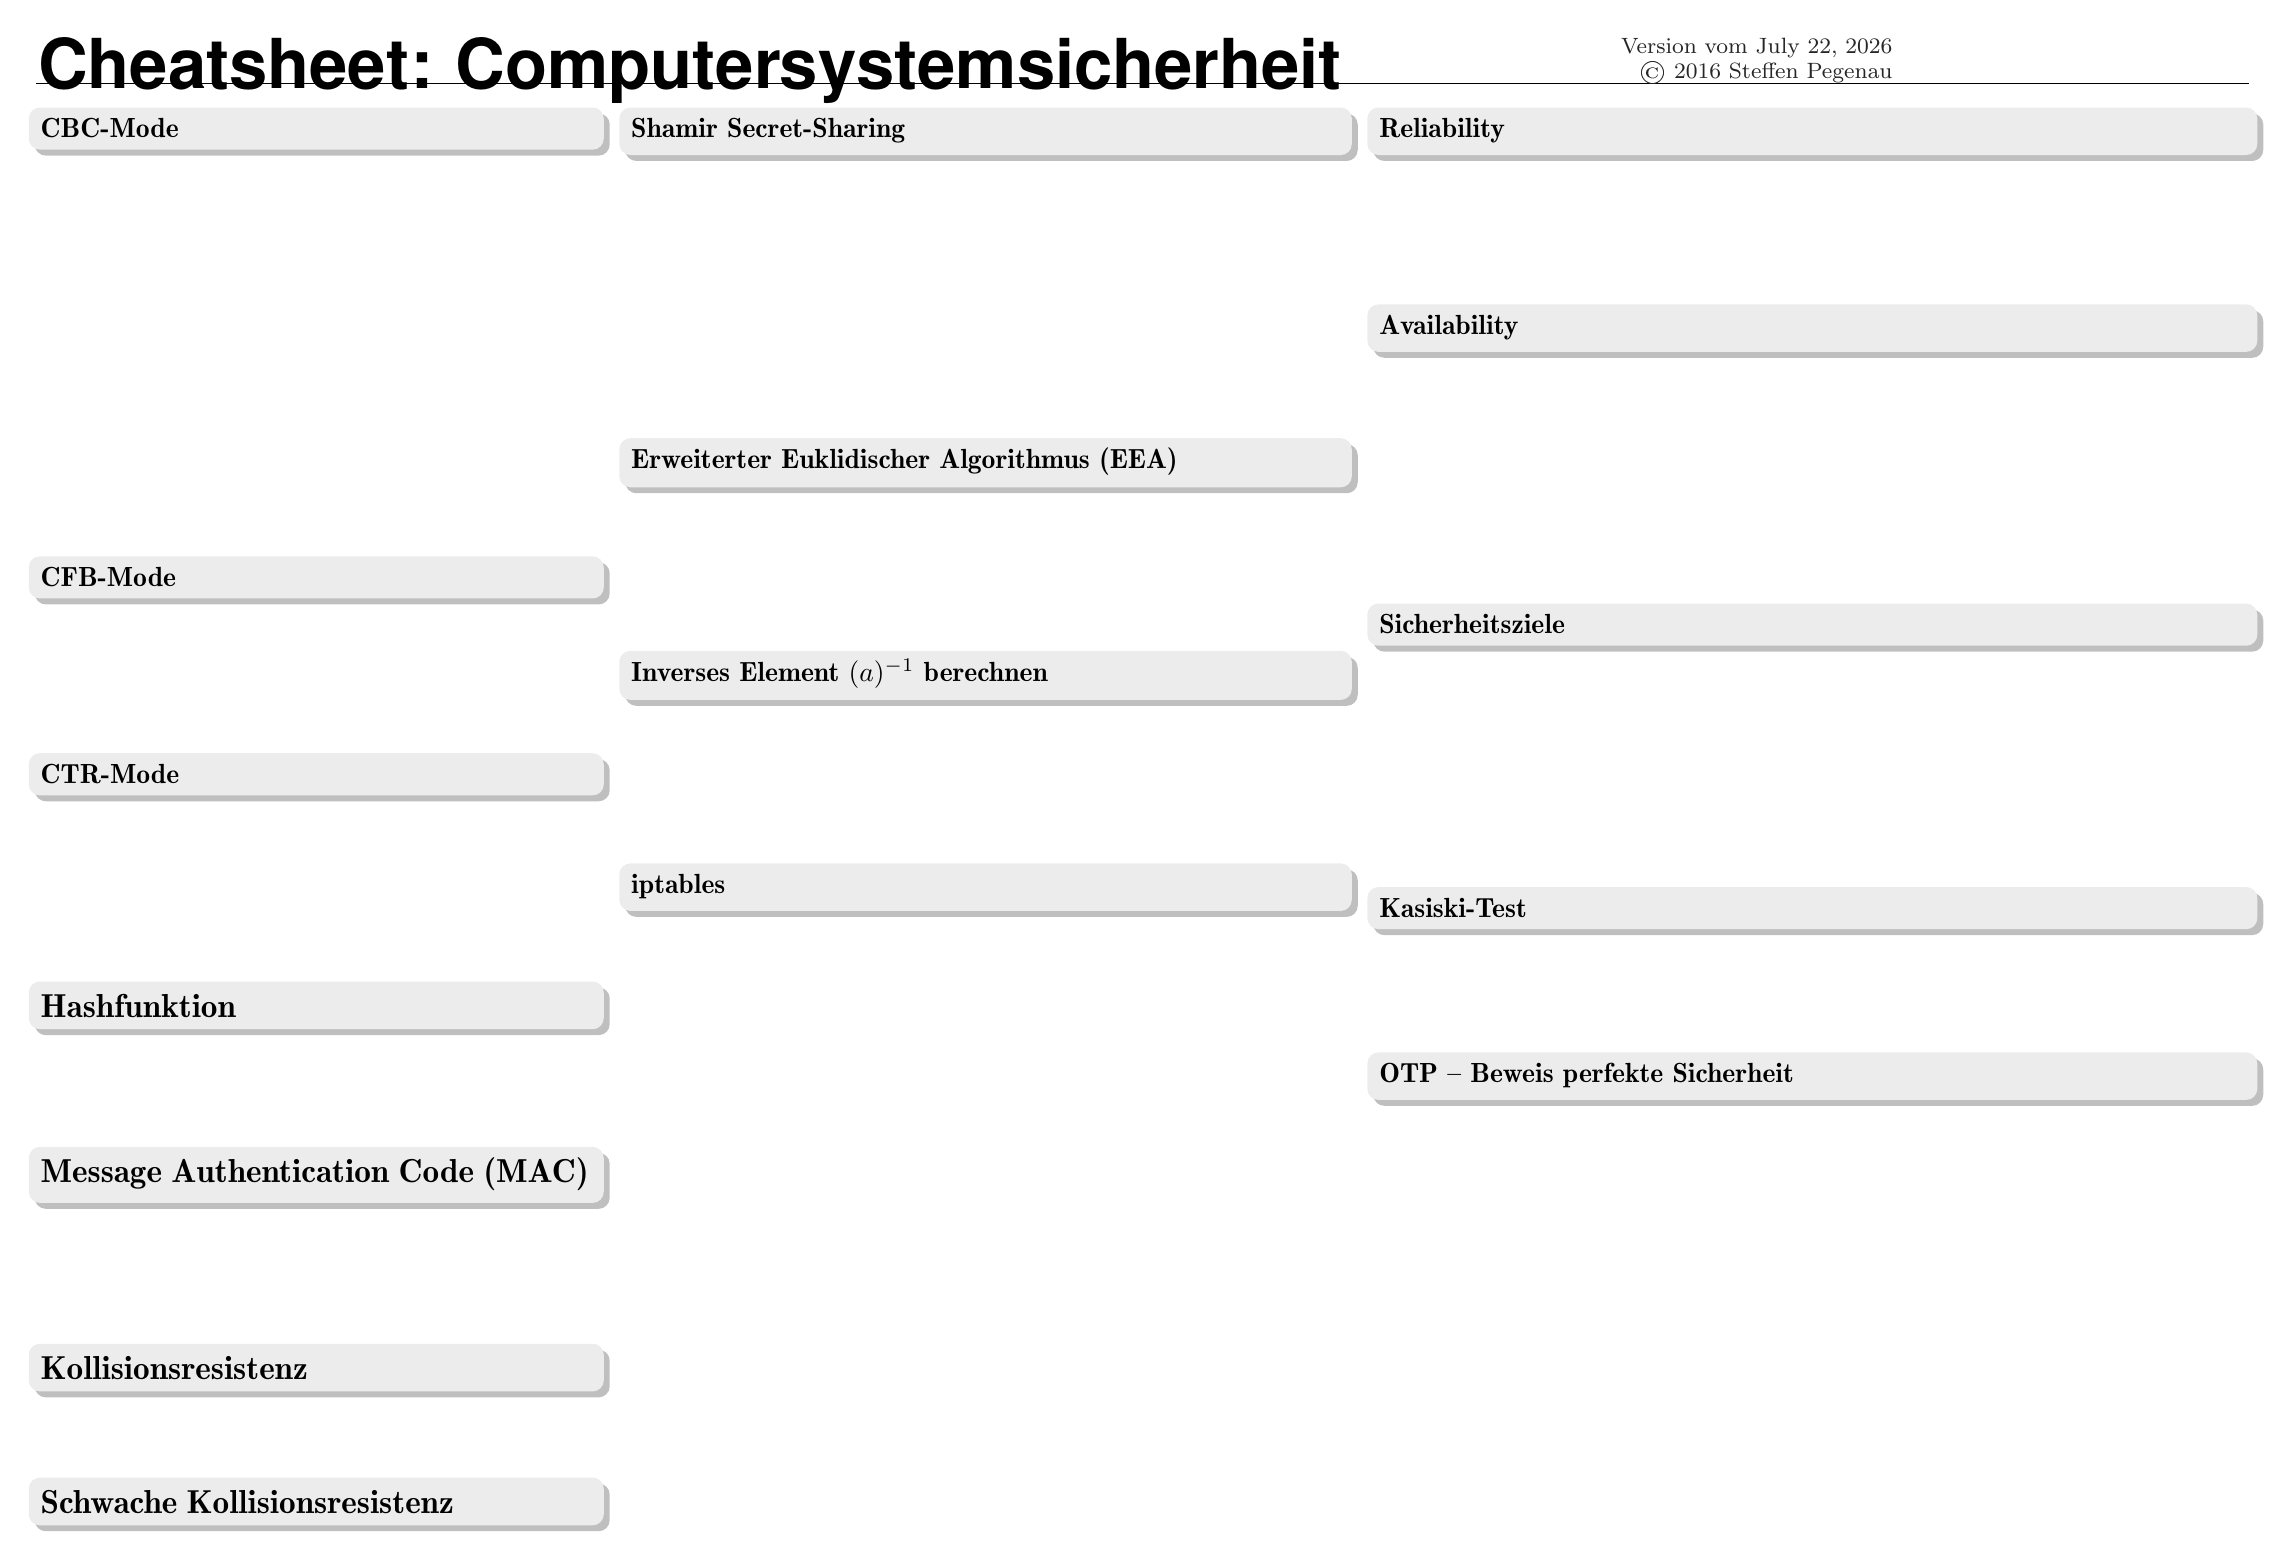
\begin{tikzpicture}
  \draw (0,1) node[anchor=north west,font=\Huge\bf\fontfamily{phv}\selectfont]{Cheatsheet: Computersystemsicherheit}
  (.1cm,.3cm) -- (28.2cm,.3cm)
  ([xshift=1mm]23.7cm,.7cm)
  node[font=\footnotesize,color=black!85,anchor=north east]{
    \copyright{} 2016 Steffen Pegenau
  }
  ++(0,.3cm)
  node[font=\footnotesize,color=black!85,anchor=north east]{
    Version vom \today
  }
  ;
  \draw
  (0,0) node[anchor=north west,text width=\breiteErsteSpalte,rounded corners,fill=gray!15,inner sep=1ex,drop shadow]
  (linksoben)
  {
   \platz
   \subsubsection*{CBC-Mode}
  }
  ++(0,-5.7cm) node[below right,text width=\breiteErsteSpalte,rounded corners,fill=gray!15,inner sep=1ex,drop shadow]
  {
    \platz
    \subsubsection*{CFB-Mode}
  }
  ++(0,-2.5cm) node[below right,text width=\breiteErsteSpalte,rounded corners,fill=gray!15,inner sep=1ex,drop shadow]
  {
    \platz
    \subsubsection*{CTR-Mode}
  }
  ++(0, -2.9cm) node[below right,text width=\breiteErsteSpalte,rounded corners,fill=gray!15,inner sep=1ex,drop shadow]
  {
    \platz
    \subsection*{Hashfunktion}
    
  }
  ++(0, -2.1cm) node[below right,text width=\breiteErsteSpalte,rounded corners,fill=gray!15,inner sep=1ex,drop shadow]
  {
    \platz
    \subsection*{Message Authentication Code (MAC)}
  }
  ++(0, -2.5cm) node[below right,text width=\breiteErsteSpalte,rounded corners,fill=gray!15,inner sep=1ex,drop shadow]
  {
    \platz
    \subsection*{Kollisionsresistenz}
  }
  ++(0, -1.7cm) node[below right,text width=\breiteErsteSpalte,rounded corners,fill=gray!15,inner sep=1ex,drop shadow]
  {
    \platz
    \subsection*{Schwache Kollisionsresistenz}
  }
;
  \draw (linksoben.north west)
  ++(7.5cm,0) node[anchor=north west,text width=\breiteZweiteSpalte,rounded corners,fill=gray!15,inner sep=1ex,drop shadow]
  (zweite-spalte)
  {
    \platz
    \subsubsection*{Shamir Secret-Sharing}
  }
  ++(0,-4.2cm) node[below right,text width=\breiteZweiteSpalte,rounded corners,fill=gray!15,inner sep=1ex,drop shadow]
  {
    \platz
    \subsubsection*{Erweiterter Euklidischer Algorithmus (EEA)}

  }
  ++(0,-2.7cm) node[below right,text width=\breiteZweiteSpalte,rounded corners,fill=gray!15,inner sep=1ex,drop shadow]
  {
    \platz
    \subsubsection*{Inverses Element $(a)^{-1}$ berechnen}
  }
  ++(0,-2.7cm) node[below right,text width=\breiteZweiteSpalte,rounded corners,fill=gray!15,inner sep=1ex,drop shadow]
  {
    \platz
    \subsubsection*{iptables}
  };
  \draw (zweite-spalte.north west)
  ++(9.50cm,0) node[below right,text width=\breiteDritteSpalte,rounded corners,fill=gray!15,inner sep=1ex,drop shadow]
  {
    \platz
    \subsubsection*{Reliability}
  }
  ++(0,-2.5cm) node[below right,text width=\breiteDritteSpalte,rounded corners,fill=gray!15,inner sep=1ex,drop shadow]
  {
    \platz
    \subsubsection*{Availability}
    
  }
  ++(0,-3.8cm) node[below right,text width=\breiteDritteSpalte,rounded corners,fill=gray!15,inner sep=1ex,drop shadow]
  {
    \platz
    \subsubsection*{Sicherheitsziele}
  }
  ++(0,-3.6cm) node[below right,text width=\breiteDritteSpalte,rounded corners,fill=gray!15,inner sep=1ex,drop shadow]
  {
    \platz
    \subsubsection*{Kasiski-Test}
  }
  ++(0,-2.1cm) node[below right,text width=\breiteDritteSpalte,rounded corners,fill=gray!15,inner sep=1ex,drop shadow]
  {
    \platz
    \subsubsection*{OTP -- Beweis perfekte Sicherheit}

  }
  ;
\end{tikzpicture}

%%% }}}
%%%%%%%%%%%%%%%%%%%%%%%%%%%%%%%%%%%%%%%%%%%%%%%%%%%%%%%%%%%%

\end{document}

%%% vim:set fdm=marker:
